\begin{frame}[t]{Which system is better, A or B?}
  \begin{center}
    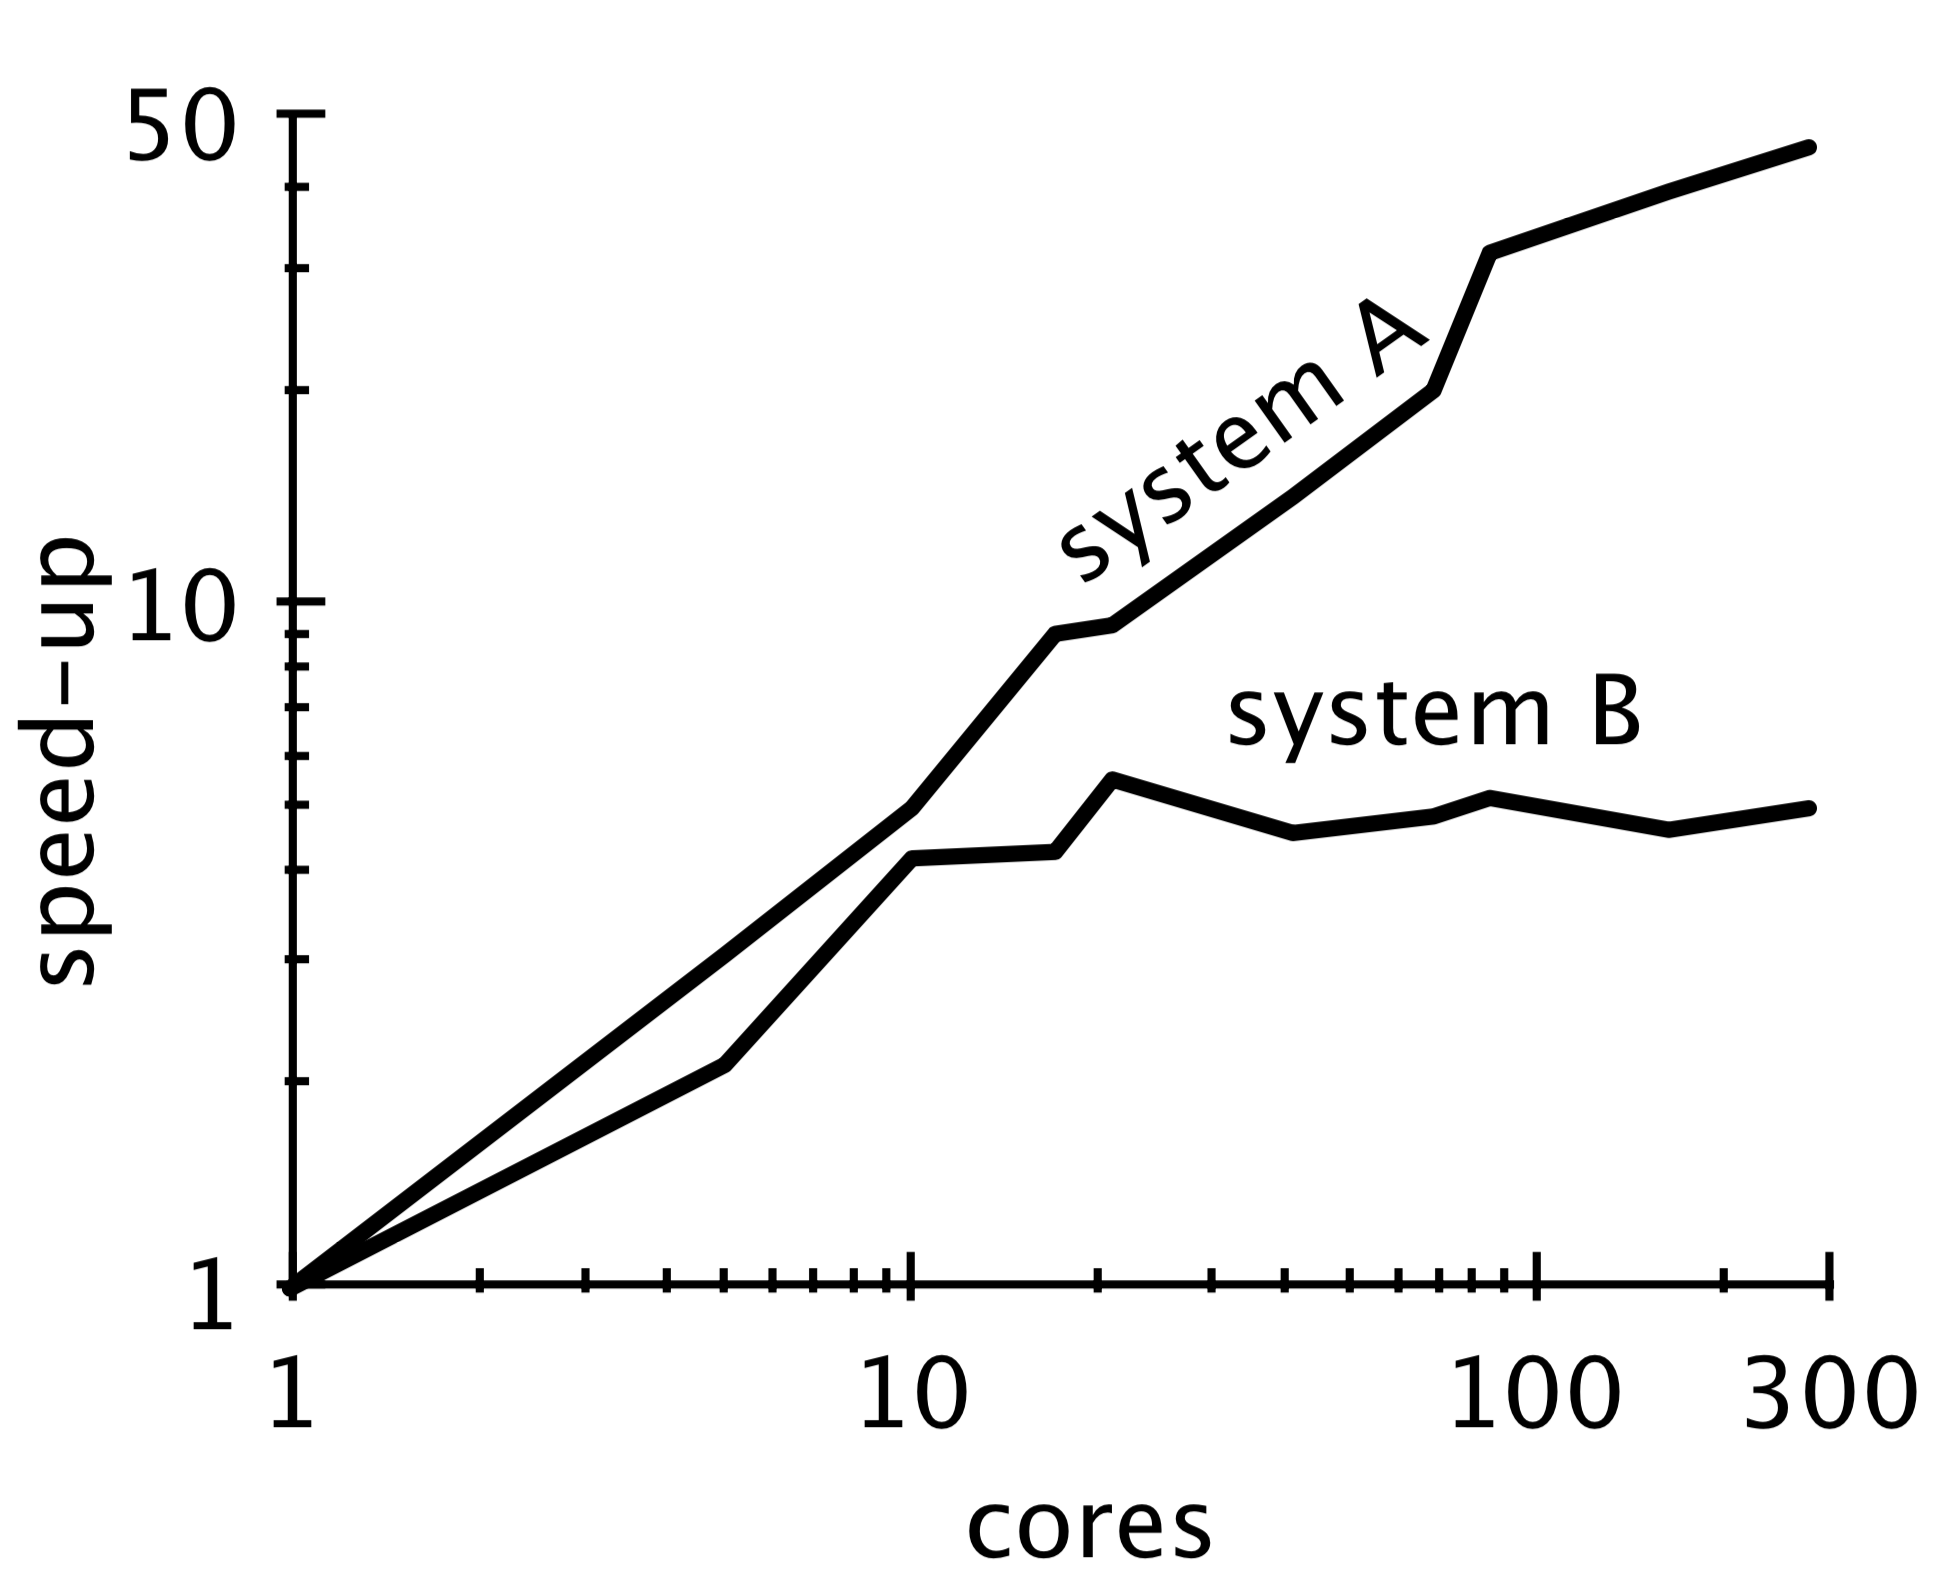
\includegraphics[width=0.76\textwidth]{scalability-1}
  \end{center}
\end{frame}

\begin{frame}[t]{What about now, A or B?}
  \begin{center}
    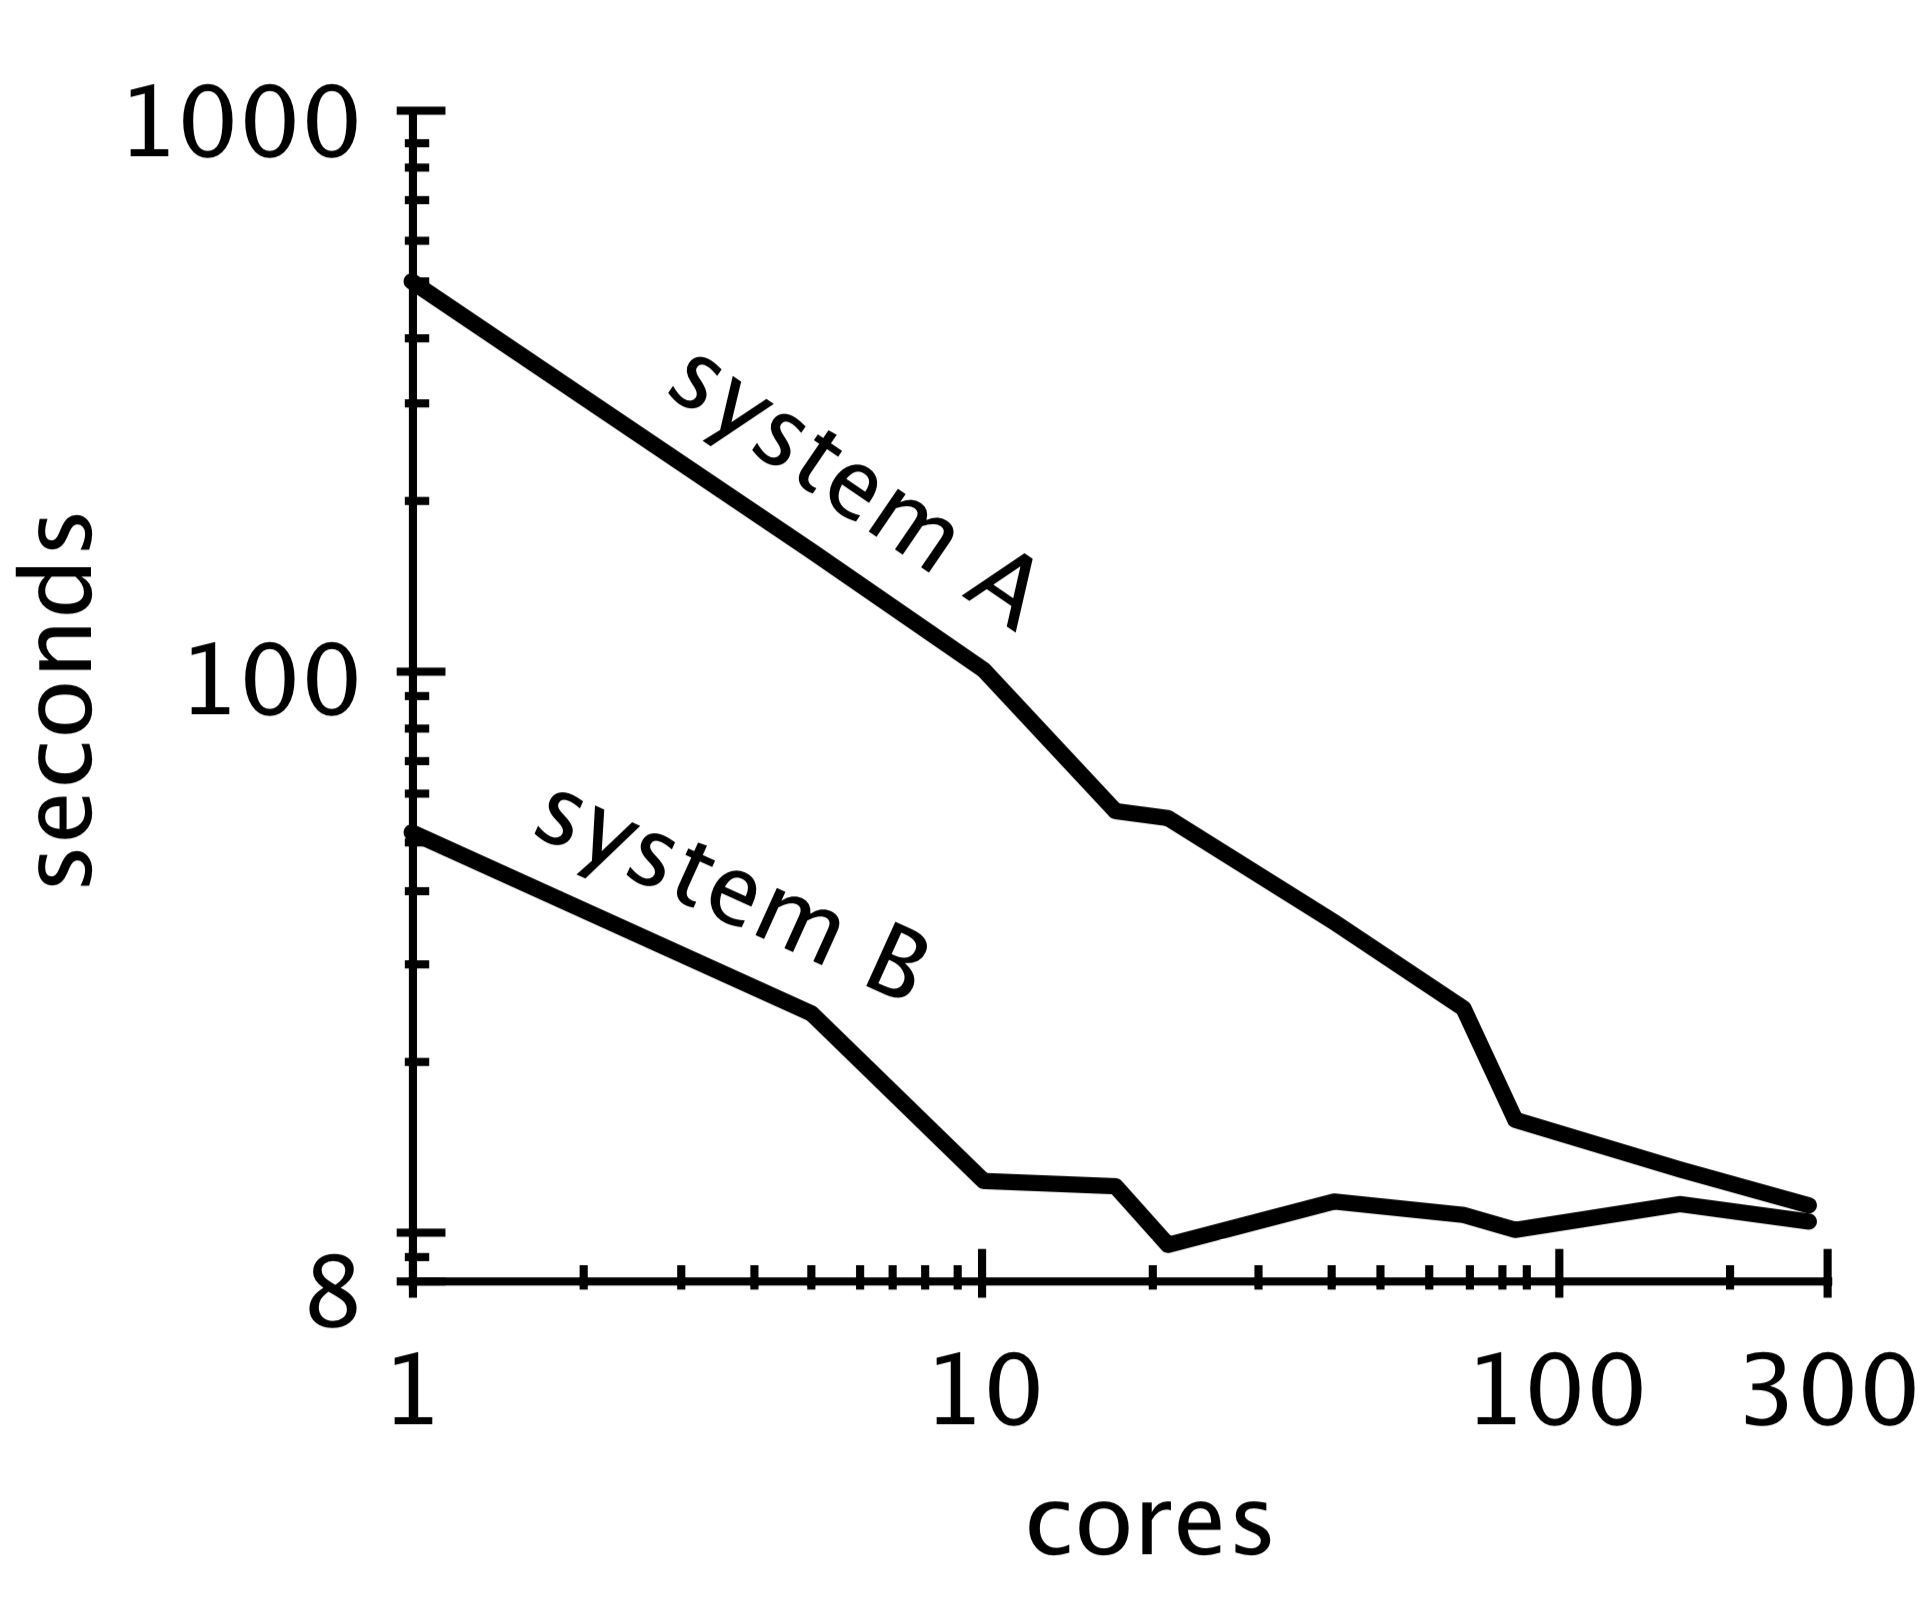
\includegraphics[width=0.76\textwidth]{scalability-2}
  \end{center}
\end{frame}

\begin{frame}[t]{Question in hand}
  \begin{center}
    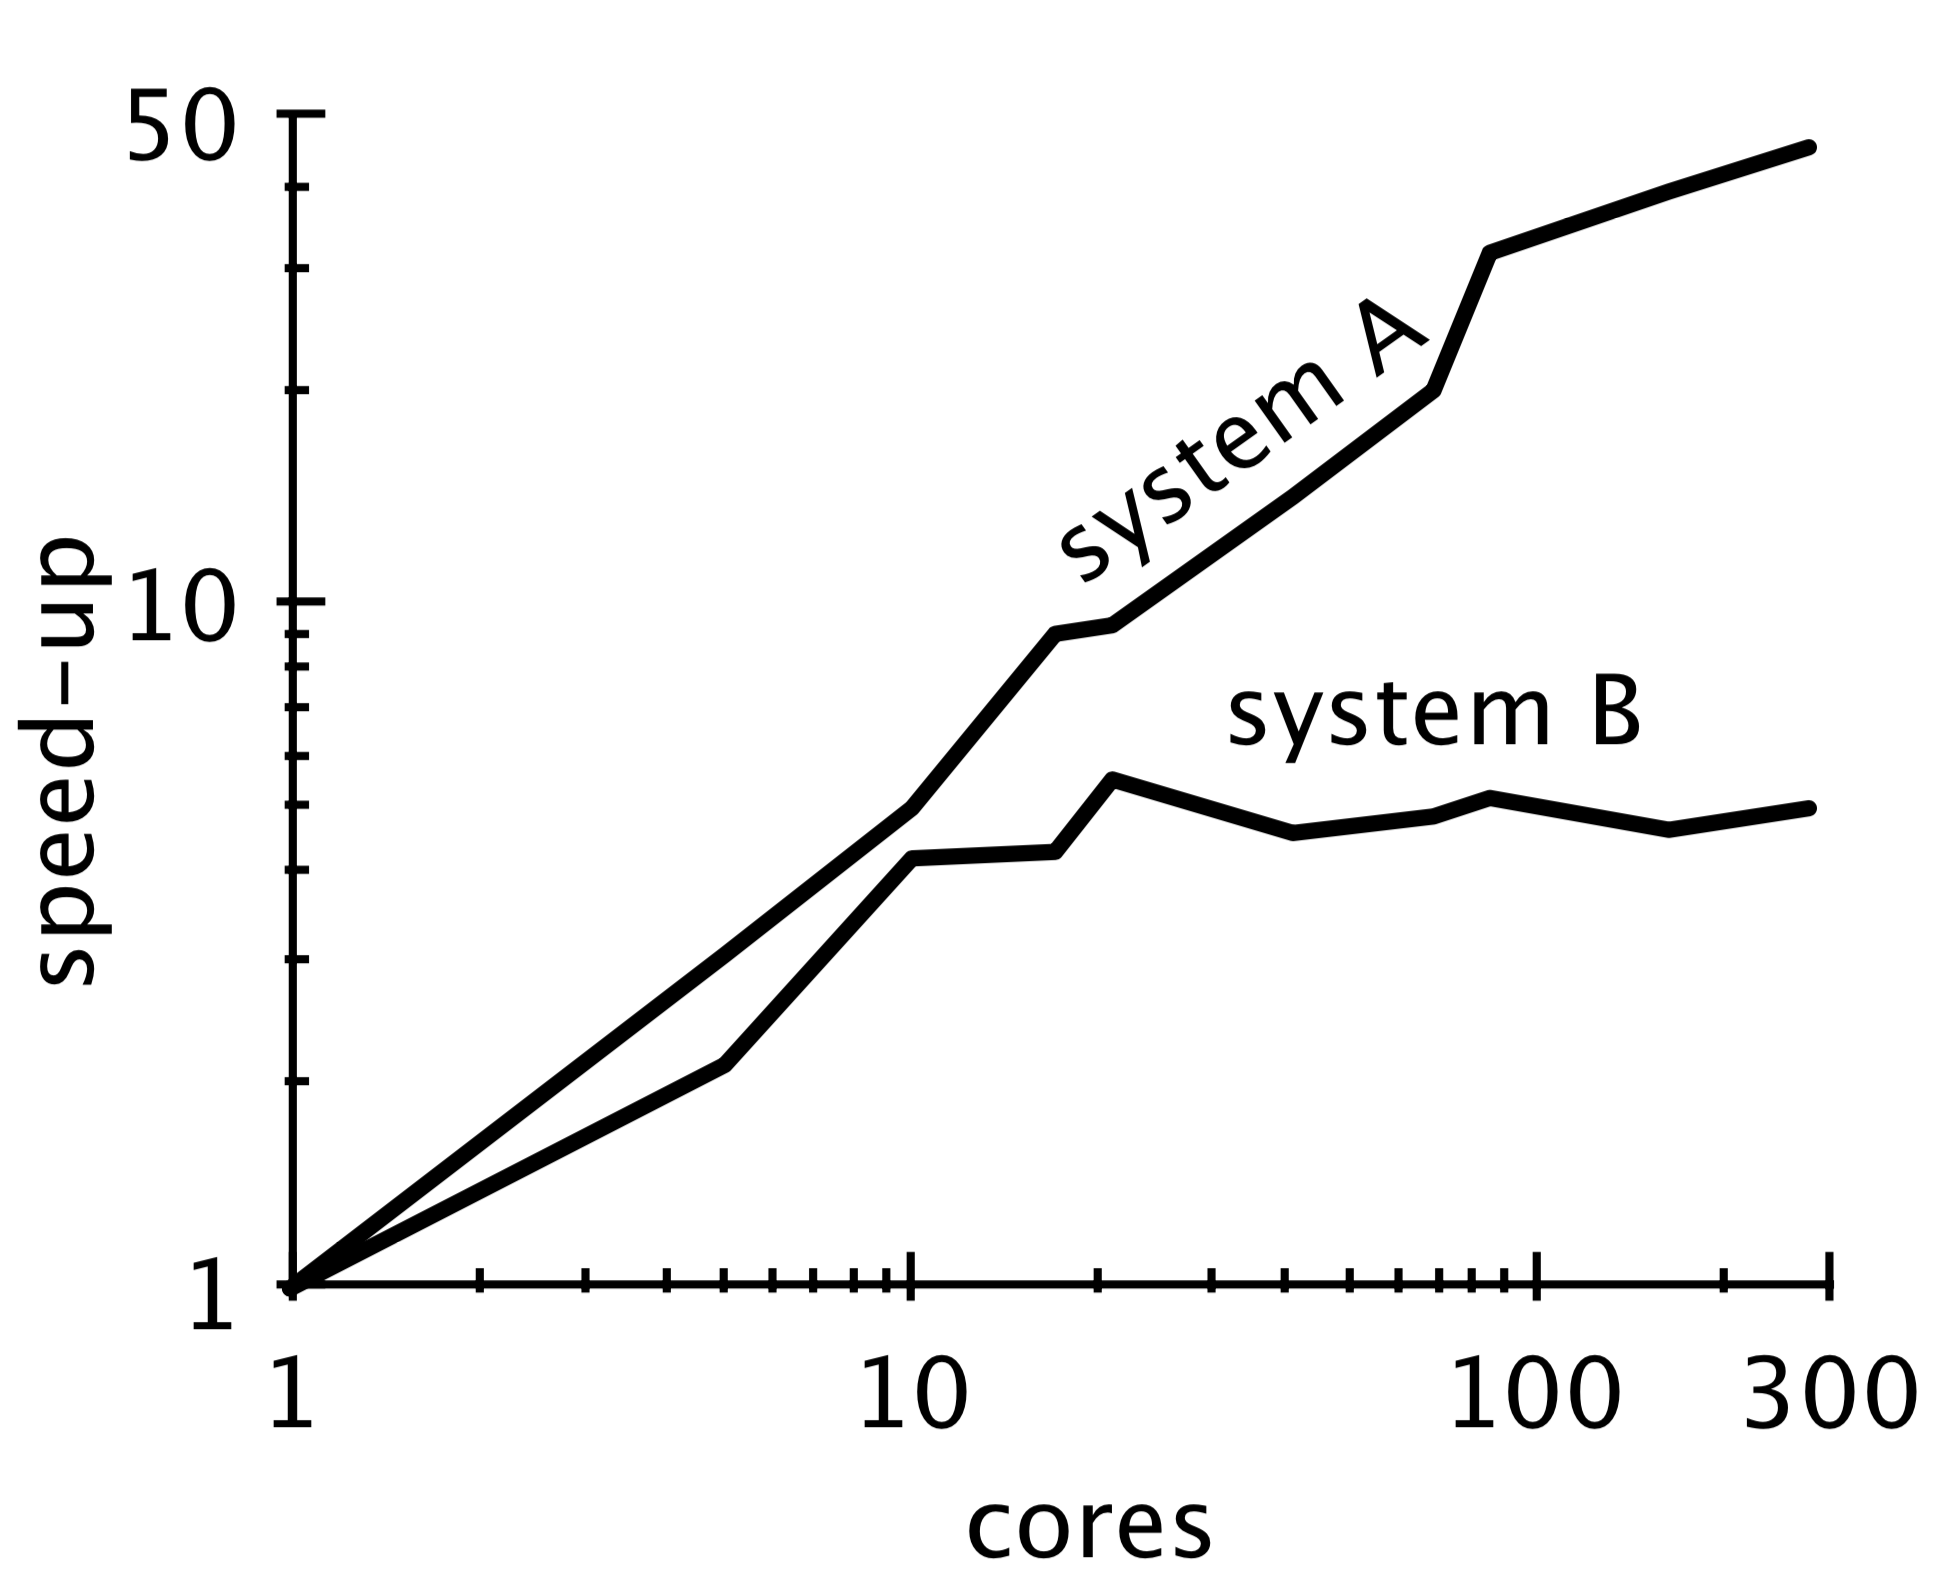
\includegraphics[width=0.42\textwidth]{scalability-1}
    \hspace{0.5cm}
    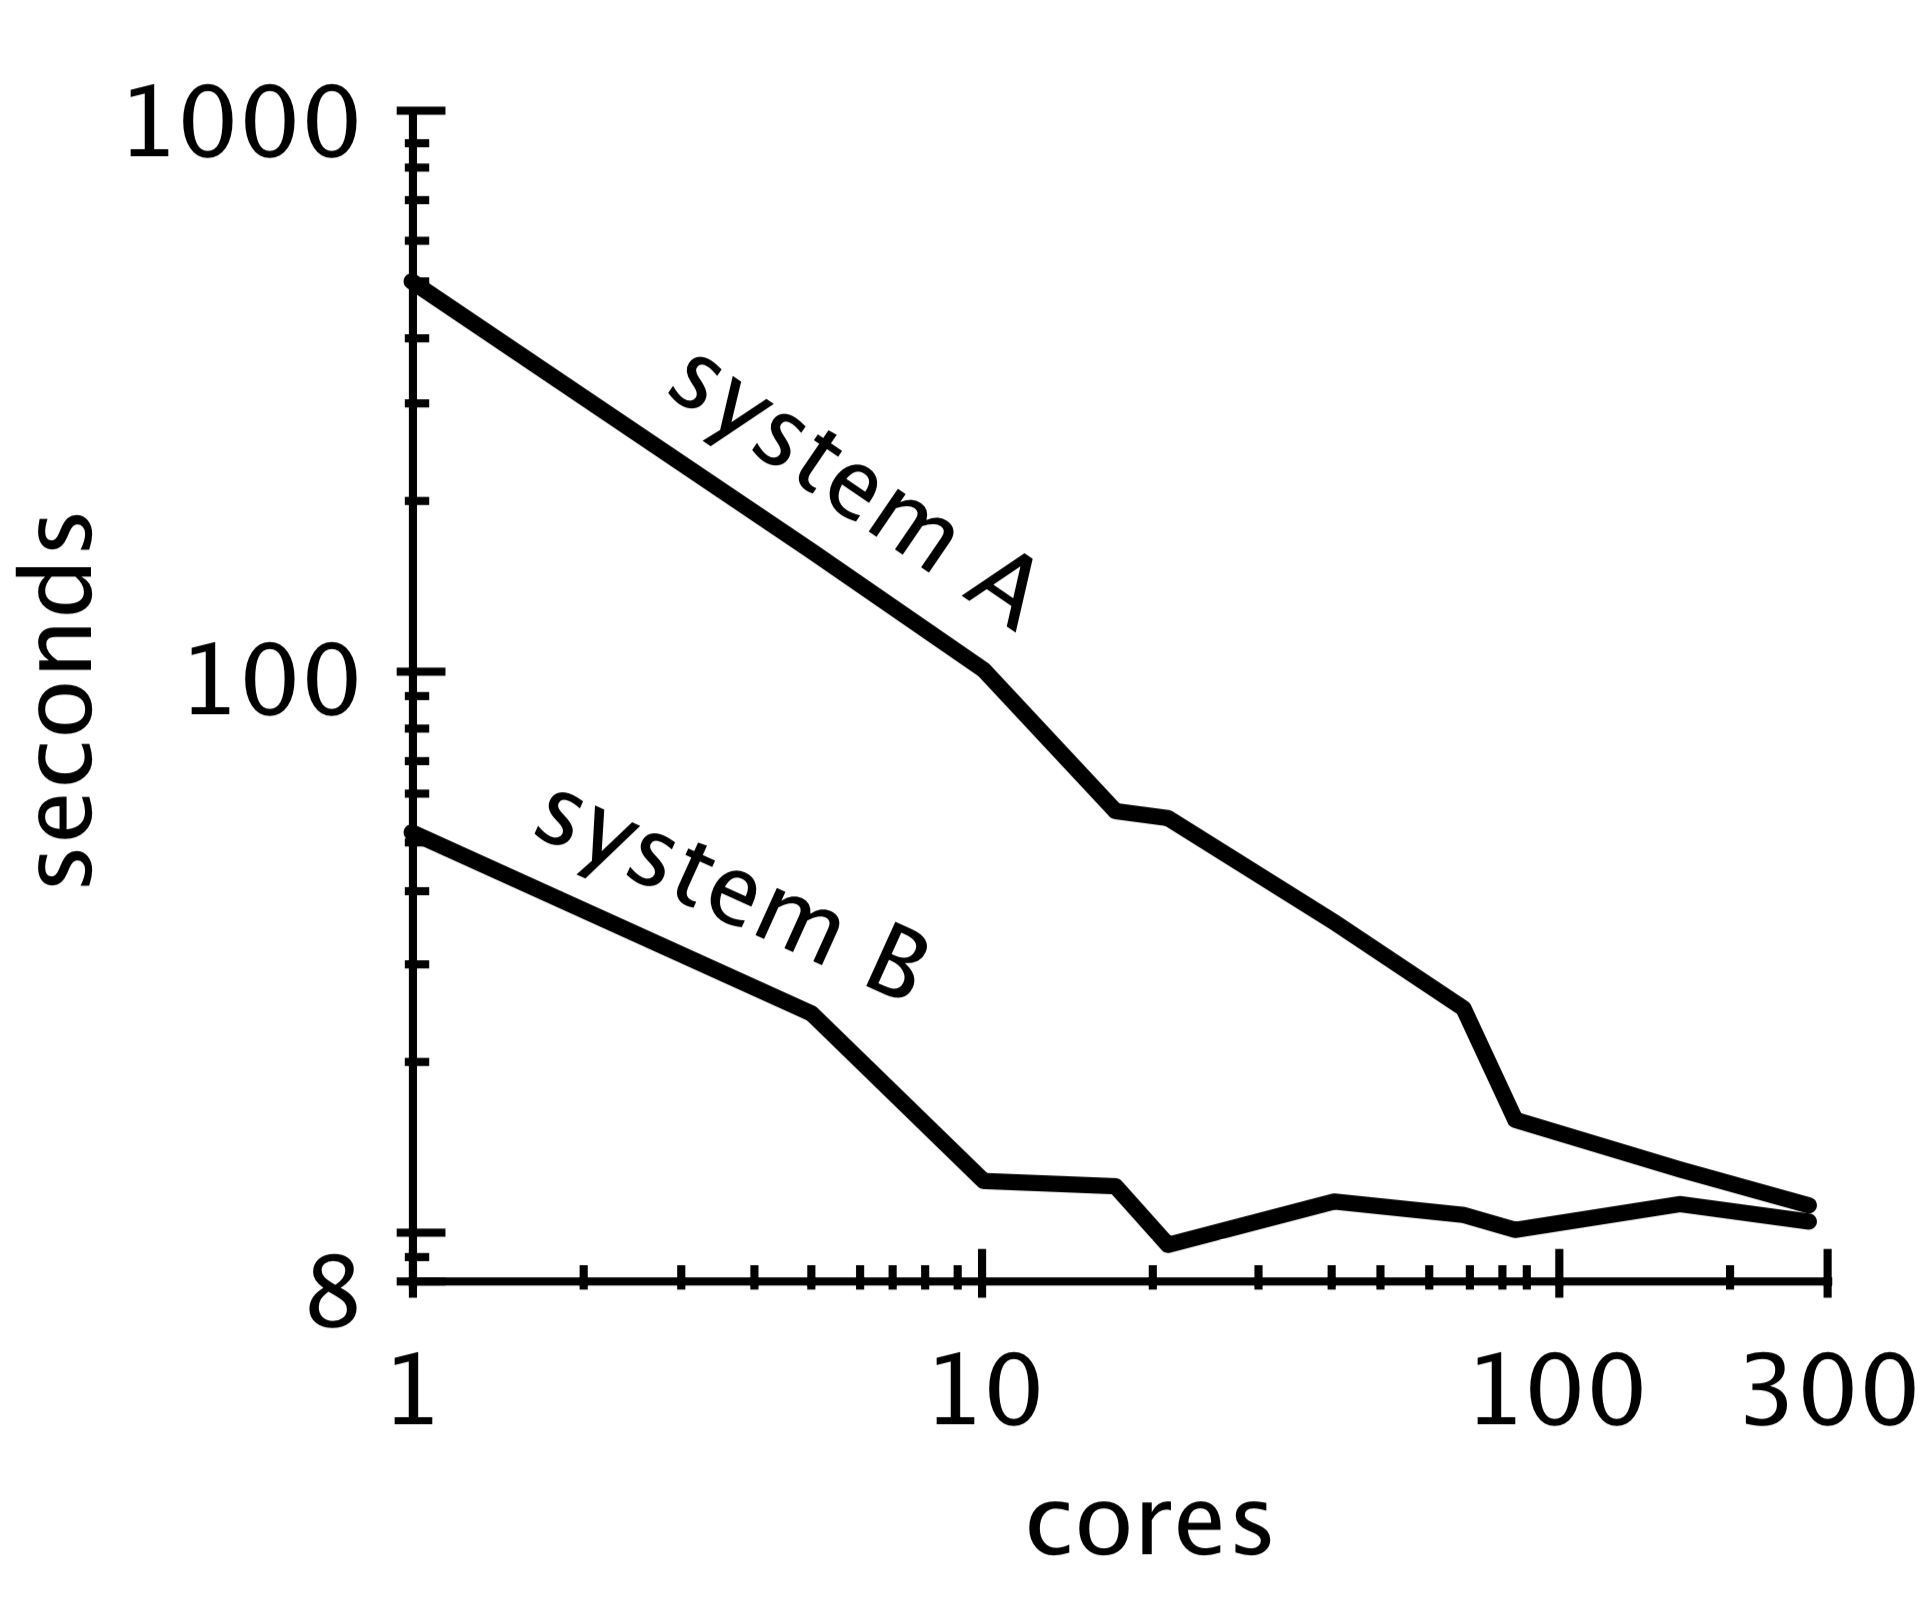
\includegraphics[width=0.42\textwidth]{scalability-2}
  \end{center}

  \begin{itemize}
    \item Scalability is often touted as an essential attribute.
    \item Absolute performance is not related to scalability.
  \end{itemize}

  \vspace{0.5cm}
  \pause

  \textit{To what degree are scalable systems truly improving performance, \\ as opposed to parallelizing overheads introduced?}

\end{frame}

\begin{frame}[t]{How can we measure?}
  \begin{center}
    \Large{"What you can't measure, you can't improve"}
  \end{center}
  \vspace{1.5cm}
  \pause
  COST - \textbf{C}onfiguration that \textbf{O}utperforms a \textbf{S}ingle \textbf{T}hread

  \vspace{1.5cm}
  Why measure against a single thread?
  \begin{itemize}
    \item Distributed systems can have huge overheads.
    \item Most systems have \textit{unbounded} COST!
    \item More optimizations can be applied 
  \end{itemize}
\end{frame}